\documentclass{../tuda-exercise}

% Title information
\version{20. November 2021}
\sheetnumber{5}

\begin{document}

  \maketitle

  \begin{task}{DrRacket installieren}
    Installieren Sie zu Beginn DrRacket von folgendem Link auf Ihrem Rechner:

    \begin{center}
      \url{https://racket-lang.org/download/}
    \end{center}

    In Abbildung \ref{fig:V1} sehen Sie, wie die Oberfläche dann aussieht. Vergewissern Sie sich,
    dass links unten (im Screenshot gelb hinterlegt) auch \textit{Advanced Student} steht.
    Andernfalls kicken Sie auf die im Bild gelb markierte Fläche und stellen es darauf um.

    \begin{figure}[h]
      \centering
      \includegraphics[width=\linewidth]{graphics/gui_drracket.png}
      \caption{Oberfläche von DrRacket}
      \label{fig:V1}
    \end{figure}
  \end{task}

  \clearpage

  \begin{note}[title=Wichtig:, color=tuda-red]
    Denken Sie an den Vertrag und die drei Tests bei jeder Funktion.
  \end{note}

  \begin{note}[title=Achtung:, color=tuda-red]
    Beachten Sie, dass ein Funktionsaufruf erwartet wird, falls Sie eine geöffnende Klammer
    schreiben. Wenn Sie das nicht beachten, erhalten Sie folgende Fehlermeldung:

    \begin{center}
      function call: expected a function after the open parenthesis, but received XYZ
    \end{center}
  \end{note}

  \begin{task}[credit=\stars{0}{3}]{Temperaturumrechnung}
    Im angloamerikanischen Maßsystem wird die Temperatur nicht wie hierzulande in Grad Celsius
    gemessen, sondern in Grad Fahrenheit. Da Sie damit nichts anfangen können, wollen Sie sich
    nun eine Funktion \inlineracket{fahr->cel} definieren, welche die aktuelle Temperatur in Grad
    Fahrenheit übergeben bekommt und in Grad Celsius umwandelt.

    \br

    \begin{note}[title=Hinweis:, color=tuda-orange]
      Für eine gegebene Temperatur \(T_F\) in Grad Fahrenheit berechnet sich die dazugehörige
      Temperatur \(T_C\) in Grad Celsius über den folgenden Zusammenhang:

      \begin{equation*}
        T_C = (T_F - 32) \cdot \frac{5}{9}
      \end{equation*}
    \end{note}

    \begin{solution}
      \lstinputlisting[style=Racket]{codes/V2_Solution.rkt}
    \end{solution}
  \end{task}

  \clearpagesolution

  \begin{task}[credit=\stars{1}{3}]{Volumen eines Tetraeders}
    Das Tetraeder ist ein Körper mit vier dreieckigen Seitenflächen. Sein Volumen berechnet sich
    über die Formel \(V(a) = \frac{\sqrt{2}}{12} a^3\), wobei \(a\) hier die Länge einer Kante
    ist. Sie sollen in dieser Aufgabe nun eine Funktion \inlineracket{tetrahedron-volume}
    schreiben, die für eine übergebene Kantenlänge \(a\) das Volumen des dazugehörigen Tetraeders
    zurückgibt. Gehen Sie dazu in folgenden Schritten vor:

    \begin{enumerate}
      \item Definieren Sie eine Funktion \inlineracket{pow3}, welche einen Parameter
      \inlineracket{x} bekommt, und den Wert \(x^3\) zurückgibt. Erstellen Sie außerdem eine
      Konstante \inlineracket{k}, mit dem Wert \(\frac{\sqrt{2}}{12}\).
      \item Nutzen Sie die zwei vorherigen Schritte, um nun die Funktion
      \inlineracket{tetrahedron-volume} zu definieren, welche nur einen Parameter
      \inlineracket{a} bekommt.
    \end{enumerate}

    \begin{solution}
      \lstinputlisting[style=Racket]{codes/V3_Solution.rkt}
    \end{solution}
  \end{task}

  \clearpage

  \begin{task}[credit=\stars{1}{3}]{Relative Lage zweier Kreise zueinander}
    Wir wollen die Lage zweier Kreise zueinander bestimmen. Definieren Sie dazu eine Prozedur
    \inlineracket{circles-position}, welche die Zahlen \inlineracket{x1, y1, r1, x2, y2, r2} in
    dieser Reihenfolge entgegennimmt und einen String zurückgibt, welche die Lage der beiden
    Kreise zueinander beschreibt. Dabei sind \inlineracket{x} und \inlineracket{y} die
    Koordinaten eines Kreismittelpunktes und \inlineracket{r} der Radius des Kreises.

    \br

    Zurückgegeben werden soll \code{\textcolor{stringcolor}{"'Intersect"'}} bei einem Schnitt der
    beiden Kreise, \code{\textcolor{stringcolor}{"'External"'}} bei keinerlei Überlappung oder
    \code{\textcolor{stringcolor}{"'Interior"'}} wenn einer der beiden Kreise vollständig im
    anderen liegt. Eine Berührung der beiden Kreise, egal ob von innen oder von außen, soll als
    Schnitt der beiden Kreise erkannt werden.

    \br

    Zum besseren Verständnis finden Sie im Anschluss an die Aufgabe ein Beispiel und die
    mathematische Konkretisierung des Sachverhalts (dabei steht \inlineracket{d} für den Abstand
    der Mittelpunkte). Bei den Kreisen \(K_1\) und \(K_2\) im Beispiel sollte
    \code{\textcolor{stringcolor}{"'Intersect"'}}, bei den Kreisen \(K_1\) und \(K_3\) sollte
    \code{\textcolor{stringcolor}{"'External"'}} und bei den Kreisen \(K_2\) und \(K_3\) sollte
    \code{\textcolor{stringcolor}{"'Interior"'}} zurückgegeben werden.

    \begin{minipage}{.45\linewidth}
      \begin{figure}[H]
        \centering
        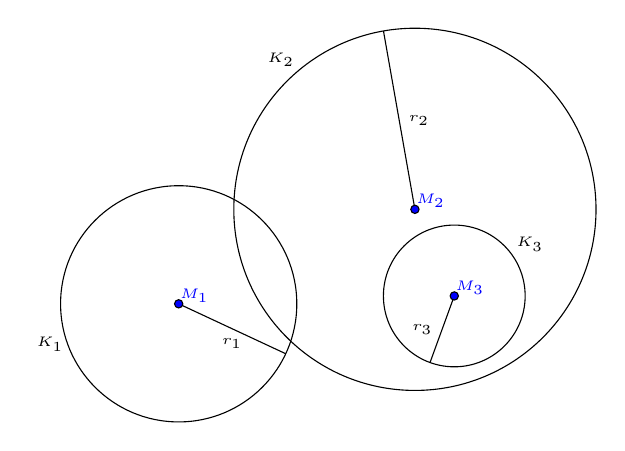
\begin{tikzpicture}
          [
          every node/.style={
            font=\tiny
          },
          center/.style={
            draw=black,
            fill=blue,
            minimum size=3pt,
            thin,
            circle,
            inner sep=0pt,
            label={[blue, label distance=-6pt]above right:#1}
          }]
          \draw (0, 0) circle (1.5cm) node[center=$M_{1}$] {} -- node[below] {$r_{1}$}
          +(-25:1.5cm) +(200:1.5cm) node[left=-2pt] {$K_{1}$};
          \draw (3, 1.2) circle (2.3cm) node[center=$M_{2}$] {} -- node[right] {$r_{2}$}
          +(100:2.3cm) +(130:2.3cm) node[above left=-2pt] {$K_{2}$};
          \draw (3.5, 0.1) circle (0.9cm) node[center=$M_{3}$] {} -- node[left] {$r_{3}$}
          +(-110:0.9cm) +(35:0.9cm) node[above right=-2pt] {$K_{3}$};
        \end{tikzpicture}
      \end{figure}
    \end{minipage}
    \hfill
    \begin{minipage}{.45\linewidth}
      \begin{equation*}
        \text{circles-position} =
        \begin{cases}
          \text{Interior}  & \text{if } d < \vert r_1 - r_2 \vert
          \\
          \text{External}  & \text{if } r_1 + r_2 < d
          \\
          \text{Intersect} & \text{otherwise}
        \end{cases}
      \end{equation*}
    \end{minipage}

    Zur Berechnung von \inlineracket{d} verwenden Sie den euklidischen Abstand der Mittelpunkte
    der zwei zu vergleichenden Kreise. Der Abstand zweier Punkt \(p_1 = (x_1, y_1)\) und \(p_2 =
    (x_2, y_2)\) ist folgendermaßen definiert \(d_{p_1, p_2} = \sqrt{(x_2 - x_1)^2 + (y_2 - y_1)
      ^2}\).

    \clearpagesolution

    \begin{solution}
      \lstinputlisting[style=Racket]{codes/V4_Solution.rkt}
    \end{solution}
  \end{task}

  \clearpagesolution

  \begin{task}[credit=\stars{1}{3}]{Euklidischer Algorithmus}
    In der folgenden Aufgabe soll das Konzept der Rekursion verinnerlicht werden. Dazu werfen wir
    einen Blick auf eine Version des euklidischen Algorithmus, welcher Ihnen vielleicht schon aus
    der Mathematik bekannt ist. Für zwei natürliche Zahlen \inlineracket{a} und \inlineracket{b}
    lässt sich mit ihm der größte gemeinsame Teiler der beiden Zahlen berechnen. Dabei geht der
    Algorithmus wie folgt vor:

    \br

    Gilt \inlineracket{b = 0} so wird \inlineracket{a} zurückgegeben, ist hingegen
    \inlineracket{a = 0} so wird \inlineracket{b} zurückgegeben. Gilt \inlineracket{a > b} so wird
    der Algorithmus mit einem neuen \(\hat{a} = a - b\) und dem "'alten"'{} \inlineracket{b}
    aufgerufen. Im anderen Fall wird der Algorithmus mit dem "'alten"'{} \(a\) und einem neuen
    \(\hat{b} = b - a\) aufgerufen. Definieren Sie eine Prozedur \inlineracket{(euclid a b)},
    welche diese Version des euklidischen Algorithmus rekursiv umsetzt.

    \begin{solution}
      \lstinputlisting[style=Racket]{codes/V5_Solution.rkt}
    \end{solution}
  \end{task}

  \clearpage

  \begin{task}[credit=\stars{1}{3}]{Listenausdrücke auswerten}
  {\large\textbf{Teil A:}}
    Werden die folgenden Ausdrücke ohne Fehler durch Racket ausgeführt? Falls nein, begründen Sie
    wo und warum es zu Problemen kommt.

    \begin{enumerate}
      \item \inlineracket{(cons 1 (cons 2 (cons 3)))}
      \item \inlineracket{(cons 1 (list 2 (list (list 3 + 4))))}
      \item \inlineracket{(list (cons empty 1) (cons 2 empty) (cons 3 empty))}
      \item \inlineracket{(first empty)}
    \end{enumerate}

    {\large\textbf{Teil B:}} Liefern die folgenden Listenausdrücke dasselbe Ergebnis zurück?

    \begin{enumerate}
      \item \inlineracket{(cons 1 (cons 2 (cons 3 empty)))} und \inlineracket{(list 1 2 3 empty)}
      \item \inlineracket{(cons (list} \code{\textcolor{stringcolor}{"'(list)"'}) } \inlineracket{empty)} und
      \inlineracket{(list} \code{\textcolor{stringcolor}{"'list"'}}  \inlineracket{empty)}
      \item \inlineracket{(list 7} \code{ \textcolor{stringcolor}{"'*"'}} \inlineracket{6}
      \code{\textcolor{stringcolor}{"'="'}} \inlineracket{42)} und \inlineracket{(cons 7 (cons}
      \code{\textcolor{stringcolor}{"'*"'}} \inlineracket{(cons 6 (cons}  \code{\textcolor{stringcolor}{"'="'}}
      \inlineracket{(list 42)))))}
    \end{enumerate}

    {\large\textbf{Teil C:}} Gehen Sie nun von folgendem Codeschnipsel aus:

    \lstinputlisting[style=Racket]{codes/V6_Task.rkt}

    Was liefern die folgenden Aufrufe zurück?

    \begin{enumerate}
      \item \inlineracket{(first (rest A))}
      \item \inlineracket{(res (first A))}
      \item \inlineracket{(append (first B) (rest (rest A)) (first A))}
    \end{enumerate}

    \begin{solution}
    {\large\textbf{Teil A:}}
      \begin{enumerate}
        \item Der Ausdruck ist inkorrekt, da \inlineracket{cons} als 2. Argument immer eine Liste
        erwartet.
        \item Der Ausdruck ist korrekt.
        \item Der Ausdruck ist inkorrekt, da \inlineracket{cons} als 2. Argument immer eine Liste
        erwartet.
        \item Der Ausdruck ist inkorrekt, da \inlineracket{first} eine nichtleere Liste erwartet.
      \end{enumerate}
      {\large\textbf{Teil B:}}
      \begin{enumerate}
        \item Nein, denn \inlineracket{(list 1 2 3)} \(\neq\) \inlineracket{(list 1 2 3}
        \code{\textcolor{keywordcolor}{'()})}.
        \item Nein, denn \inlineracket{(list (list} \code{\textcolor{stringcolor}{"'(list )"'}}
        \inlineracket{))} \(\neq\) \inlineracket{(list} \code{\textcolor{stringcolor}{"'list"'}
        \textcolor{keywordcolor}{'()})}
        \item Ja, denn \inlineracket{(list 7} \code{\textcolor{stringcolor}{"'*"'}} \inlineracket{6}
        \code{\textcolor{stringcolor}{"'="'}} \inlineracket{42)} = \inlineracket{(list 7}
        \code{\textcolor{stringcolor}{"'*"'}} \inlineracket{6}
        \code{\textcolor{stringcolor}{"'="'}} \inlineracket{42)}
      \end{enumerate}
      {\large\textbf{Teil C:}}
      \begin{enumerate}
        \item \inlineracket{(list 7)}
        \item \code{\textcolor{keywordcolor}{'()}} (leere Liste)
        \item Es wird eine Fehlermeldung geworfen, da \inlineracket{append} als Argumente Listen
        erwartet. Jedoch ist
        das erste Argument eine Zahl.
      \end{enumerate}
    \end{solution}
  \end{task}

  \begin{task}[credit=\stars{1}{3}]{Strukturausdrücke auswerten}
    Gegeben sei folgende Strukturdefinition:

    \lstinputlisting[style=Racket]{codes/V7_Task.rkt}

    Was liefern die folgenden Aufrufe zurück?

    \begin{enumerate}
      \item \inlineracket{(my-pair? (make-my-pair} \code{\textcolor{stringcolor}{"'a"'}
      \textcolor{stringcolor}{"'b"'}))}
      \item \inlineracket{(make-my-pair 1 (make-my-pair 2 empty))}
      \item \inlineracket{(* (my-pair-two (make-my-pair 1 2))(my-pair-one (make-my-pair 3 4)))}
    \end{enumerate}

    \begin{solution}
      \begin{enumerate}
        \item Wahr, da dies ein Struct von my-pair ist.
        \item \inlineracket{(make-my-pair 1 (make-my-pair 2 empty))}
        \item 6
      \end{enumerate}

      \begin{note}[title=Information:]
        Ein Struct ist eine Strukturtypbeschreibung mit null oder mehr Feldern. Structs werden
        mit einer bestimmten Syntax definiert, die es ermöglicht Prozeduren für die Erstellung
        von Instanzen vom Typ des Structs und Prozeduren für den Zugriff auf die Felder dieser
        Instanzen einzusetzen.

        \begin{table}[H]
          \centering
          \begin{tabular}{p{10em}p{20em}p{16em}}
            \toprule
            \textbf{Befehl} & \textbf{Syntax} & \textbf{Beispiel}
            \\\midrule
            Instanziierung
            & \inlineracket{(define-struct structname (field1 field2 ...))}
            & \inlineracket{(define-struct point (x y))}
            \\
            Zugriff auf ein Feld des Structs
            & \inlineracket{(structname-fieldname element)}
            & \inlineracket{(point-x point1}\footnote{Angenommen \inlineracket{point1} ist eine
            Struktur von Typ \inlineracket{point}})
            \\
            Überprüfung, ob ein Element vom Typ Struktur X ist
            & \inlineracket{(structname? element)}
            & \inlineracket{(point? point1)} (Gibt in diesem Fall \inlineracket{\#true} zurück)
            \\\bottomrule
          \end{tabular}
          \caption{Einige Befehle von Strukturtypen}
        \end{table}
      \end{note}
    \end{solution}
  \end{task}

  \clearpagesolution

  \begin{task}[credit=\stars{1}{3}]{Listen in Strukturen}
    Gegeben ist ein Struct-Typ \inlineracket{abc} mit zwei Feldern \inlineracket{a} und
    \inlineracket{b}. Definieren Sie eine Funktion \inlineracket{foo} mit einem Parameter
    \inlineracket{p}. Falls \inlineracket{p} vom Typ \inlineracket{abc} und zudem der Wert im
    Feld \inlineracket{b} von \inlineracket{p} eine Liste ist, liefert \inlineracket{foo} eine
    Liste zurück, deren erstes Element der Wert von Feld \inlineracket{a} in \inlineracket{p}
    ist,und der Rest der zurückgelieferten Liste ist die Liste im Feld \inlineracket{b} von
    \inlineracket{p} (also eine Liste in der Liste). Andernfalls liefert \inlineracket{foo}
    einfach \inlineracket{false} zurück.

    \begin{solution}
      \lstinputlisting[style=Racket]{codes/V8_Solution.rkt}
    \end{solution}
  \end{task}

  \begin{task}[credit=\stars{2}{3}]{Suche in Zahlenliste}
    \label{task:V9}
    Definieren Sie eine Funktion \inlineracket{contains-x?}. Diese bekommt eine Liste und eine
    Zahl übergeben und liefert genau dann \inlineracket{true} zurück, wenn die übergebene Zahl
    mindestens einmal in der übergebenen Liste vorkommt.

    \begin{solution}
      \lstinputlisting[style=Racket]{codes/V9_Solution.rkt}

      \clearpage

      \paragraph{Alternative}

      Der alternative Lösungsvorschlag stammt von Kim Berninger.
      \lstinputlisting[style=Racket]{codes/V9_Solution_Alternative.rkt}
    \end{solution}
  \end{task}

  \begin{task}[credit=\stars{2}{3}]{Duplikate in Zahlenliste}
    \label{task:V10}
    Definieren Sie eine Prozedur \inlineracket{duplicates?} mit einem Parameter
    \inlineracket{lst}, die genau dann \inlineracket{true} zurückliefert, wenn eine Zahl mehr als
    einmal in \inlineracket{lst} vorkommt.

    \begin{note}[title=Hinweis:, color=tuda-orange]
      Können Sie hier vielleicht Ihre Funktion aus Aufgabe \hyperref[task:V9]{V9} verwenden?
    \end{note}

    \begin{solution}
      \lstinputlisting[style=Racket]{codes/V10_Solution.rkt}

      \clearpage

      \paragraph{Alternative}

      Der alternative Lösungsvorschlag stammt von Kim Berninger.
      \lstinputlisting[style=Racket]{codes/V10_Solution_Alternative.rkt}
    \end{solution}
  \end{task}

  \clearpagesolution

  \begin{task}[credit=\stars{3}{3}]{Verschachtelte Listen}
    Definieren Sie eine Prozedur \inlineracket{duplicates-deep?} mit einem Parameter
    \inlineracket{deep-lst}. Es wird erwartet, dass \inlineracket{deep-lst} entweder eine Zahl
    oder eine Liste ist, deren Elemente wiederum Zahlen oder Listen sind usw. (Liste von Listen
    von Zahlen). Die Prozedur \inlineracket{duplicates-deep?} soll \inlineracket{true} oder
    \inlineracket{false} zurückliefern, und zwar \inlineracket{true} genau dann, wenn
    mindestens eine Zahl mehr als einmal vorkommt.

    \begin{note}[title=Hinweis:, color=tuda-orange]
      Schreiben Sie sich eine Hilfsfunktion \inlineracket{collect} mit zwei Parametern
      \inlineracket{lst} und \inlineracket{oracle}. Nutzen Sie \inlineracket{oracle} als
      Akkumulator in dem Sie alle bereits vorgekommenen Zahlen in \inlineracket{oracle} speichern.
      Machen Sie also aus der verschachtelten Liste wieder eine normale Liste mithilfe von
      \inlineracket{collect}. Die Funktion aus  \hyperref[task:V10]{V10} kann Ihnen hier sehr
      hilfreich sein.
    \end{note}

    \begin{solution}
      \lstinputlisting[style=Racket]{codes/V11_Solution.rkt}

      \clearpage

      \paragraph{Alternative}

      Der alternative Lösungsvorschlag stammt von Kim Berninger.
      \lstinputlisting[style=Racket]{codes/V11_Solution_Alternative.rkt}

      \begin{note}[title=Information:]
        Lokale Definitionen haben zwei wichtige Funktionen: Sie bieten lokale Namen für
        Zwischenwerte, was nützlich ist, um komplizierte Ausdrücke in eine Reihe von einfacheren
        Ausdrücken aufzuteilen. Außerdem bieten sie eine Möglichkeit, die Ergebnisse von
        Berechnungen mehrfach zu nutzen (anstatt denselben Ausdruck mehrmals zu berechnen).

        \br

        Als Alternative können globale Definitionen zu demselben Zweck verwendet werden.
      \end{note}
    \end{solution}
  \end{task}

  \clearpagesolution

  \begin{task}[credit=\stars{3}{3}]{Arithmetisches Mittel}
    Gegeben seien folgende Strukturdefinition:

    \lstinputlisting[style=Racket]{codes/V12_Task.rkt}

    Eine Person hat ein Alter (als Zahl) und ein Geschlecht (als String). Ein Student wiederum
    besteht aus einer Person (vorheriges Struct) und einer Matrikelnummer (ein String).

    \br

    Definieren Sie nun eine Funktion \inlineracket{mean-of-ages}. Diese bekommt eine Liste von
    Studenten übergeben und gibt das arithmetische Mittel ihrer Alter zurück.

    \begin{note}[title=Hinweis:, color=tuda-orange]
      Das arithmetische Mittel \(\bar{x}\) berechnen Sie für \(n\) Alter \(x_1, ..., x_n\)
      mithilfe von:

      \begin{equation*}
        \bar{x} = \frac{1}{n} \sum_{i = 1}^n x_i = \frac{x_1 + ... + x_n}{n}
      \end{equation*}
    \end{note}

    \clearpagesolution

    \begin{solution}
      \lstinputlisting[style=Racket]{codes/V12_Solution.rkt}
    \end{solution}
  \end{task}
\end{document}
